%%%%%%%%%%%%%%%%%%%%%%%%%%%%%%%%%%%%%%%%%
% Short Sectioned Assignment
% LaTeX Template
% Version 1.0 (5/5/12)
%
% This template has been downloaded from:
% http://www.LaTeXTemplates.com
%
% Original author:
% Frits Wenneker (http://www.howtotex.com)
%
% License:
% CC BY-NC-SA 3.0 (http://creativecommons.org/licenses/by-nc-sa/3.0/)
%
%%%%%%%%%%%%%%%%%%%%%%%%%%%%%%%%%%%%%%%%%

%----------------------------------------------------------------------------------------
%	PACKAGES AND OTHER DOCUMENT CONFIGURATIONS
%----------------------------------------------------------------------------------------

\documentclass[paper=a4, fontsize=11pt]{scrartcl} % A4 paper and 11pt font size

\usepackage[T1]{fontenc} % Use 8-bit encoding that has 256 glyphs
\usepackage{fourier} % Use the Adobe Utopia font for the document - comment this line to return to the LaTeX default
\usepackage[english]{babel} % English language/hyphenation
\usepackage{amsmath,amsfonts,amsthm} % Math packages

\usepackage{lipsum} % Used for inserting dummy 'Lorem ipsum' text into the template

\usepackage{graphicx}
\usepackage{subcaption}
\usepackage[hidelinks]{hyperref}
\usepackage[utf8]{inputenc} 

\usepackage[toc,page]{appendix} 
\usepackage{pdfpages}

\usepackage{sectsty} % Allows customizing section commands
\allsectionsfont{\centering \normalfont\scshape} % Make all sections centered, the default font and small caps

\usepackage{fancyhdr} % Custom headers and footers
\pagestyle{fancyplain} % Makes all pages in the document conform to the custom headers and footers
\fancyhead{} % No page header - if you want one, create it in the same way as the footers below
\fancyfoot[L]{} % Empty left footer
\fancyfoot[C]{} % Empty center footer
\fancyfoot[R]{\thepage} % Page numbering for right footer
\renewcommand{\headrulewidth}{0pt} % Remove header underlines
\renewcommand{\footrulewidth}{0pt} % Remove footer underlines
\setlength{\headheight}{13.6pt} % Customize the height of the header

\numberwithin{equation}{section} % Number equations within sections (i.e. 1.1, 1.2, 2.1, 2.2 instead of 1, 2, 3, 4)
\numberwithin{figure}{section} % Number figures within sections (i.e. 1.1, 1.2, 2.1, 2.2 instead of 1, 2, 3, 4)
\numberwithin{table}{section} % Number tables within sections (i.e. 1.1, 1.2, 2.1, 2.2 instead of 1, 2, 3, 4)

\setlength\parindent{0pt} % Removes all indentation from paragraphs - comment this line for an assignment with lots of text

%----------------------------------------------------------------------------------------
%	TITLE SECTION
%----------------------------------------------------------------------------------------

\newcommand{\horrule}[1]{\rule{\linewidth}{#1}} % Create horizontal rule command with 1 argument of height

\title{	
\normalfont \normalsize 
\textsc{Aalborg University, Electronic Systems} \\ [25pt] % Your university, school and/or department name(s)
\horrule{0.5pt} \\[0.4cm] % Thin top horizontal rule
\huge Field Studies \\ % The assignment title
\horrule{2pt} \\[0.5cm] % Thick bottom horizontal rule
}

\date{\normalsize\today} % Today's date or a custom date

\begin{document}
\graphicspath{{figures/}}

\maketitle % Print the title

%----------------------------------------------------------------------------------------
%	PROBLEM 1
%----------------------------------------------------------------------------------------

\section{Purpose}
The purpose of the studies was to understand how nurses and surgeons train to operate a da Vinci robot and perform robot assisted minimal invasive surgery (RAMIS), as well as to asses what must be included in an surgery scenario.  Finally an evaluation of the finished product created is conducted on the basis of these interviews. 

\section{Method}
We observed a training session at MIUC followed by a semi-structured interview with Jane Petersson and Johan Poulsen to get an understanding of RAMIS and how surgeons practise. Furthermore, we performed a semi-structured interview with first assistant nurse Jane Petersson who is in charge of training nurses to handle the robot and how to act in a team environment.\\

A contextual inquiry is conducted to collect information resulting in different analysis models.
To analyse and retrieve information in the matter the main method used is a contextual inquiry. This includes the different analysing models and interviews. We observed a robot assisted surgery at Aalborg University Hospital performed on a living human being.

The observation team took both pictures, notes, and some video from the operation. These illustrate the tasks and teamwork necessary to perform such an operation and were used to create different models used in contextual inquiries. The models used are; a physical model showing the layout of the room, a sequence model to clarify the work flow, and an artefact model showing objects used during the procedure.\\

To evaluate the simulation created, an expert review was conducted with both Jane Petersson and Johan Poulsen.  They were both introduced to the simulation and virtual reality and were able to try the simulation. Afterwards a scripted interview was conducted. The script for this is shown in \autoref{sec:interview_script}.

\section{Results}
The results are split into three sections; one for the surgeon training at MIUC, one for the other interview with Jane Petersson regarding team training and the last for the expert review of the simulation.

\subsection{Surgeon Training at MIUC}
The training sessions at MIUC varies depending on the skill level of the participants. In cases with skilled participants, the students takes on the role as instructors to help guide during the training session. This is beneficial as the surgeon often will be in charge of during surgery.

During the interview, Jane Petersson explained that during team training a surgeon will operate the robot while making calls for the nurses in training to do. The individual tasks for the nurses depends on their current role and what they are studying to become. For instance, a first assistant nurse is the one who assists the surgeon inside of the patient. In general, the training focus highly on getting familiar with the robot and how it operates during surgery. One particular task is important for the nurses to learn - how to dock the robot. As stated by both Jane Petersson and Johan Poulsen, ensuring that the robot is rightfully docked is key to enable the surgeon full movability of the robot. Johan Poulsen also expressed the importance of sterility of staff and tools, however in a VR simulated environment errors can be made without it causing complications which is beneficial for the learning process.

\subsection{Interview with Jane Petersson}
One of the most important things during surgery and training is the emergency handling, however this requires extensive knowledge of the robot and tools. Another very important task is the placement of the robot arms because collisions during surgery can be very dangerous. Sometimes the surgeons adjust the arms manually.

In general, the training is for hands on experience with the robot and individual instruments, in preparation for a real surgery.

The team training consists of:
\begin{itemize}
  \item First assistant nurse - Sterile, assists the surgeon inside the patient's body.
  \item Scrub nurse - Sterile, prepare unpacked tools for the first assistant nurse.
  \item Circulating nurse - Not sterile, unpacks tools, and can go outside the sterile area.
\end{itemize}  

During training, on the first day Jane Petersson starts by talking and showing how tasks are done, students observe. On the second day, students are expected to do most of the tasks themselves. At the end of the second day, Jane Petersson sabotages some of the equipment and the students have to find and fix it. Any mistakes done by the students are used for learning purpose. At the beginning of the training, Jane Petersson makes most of the decisions, however later the surgeon is expected to take the lead.

\subsection{Contextual Inquiry}
The physical model shows the layout of the operation room and the personnel's workspaces. The figure includes doors and their movement as well as other objects. The layout is shown in \autoref{fig:layout}.

\begin{figure}[hpbt]
	\centering
	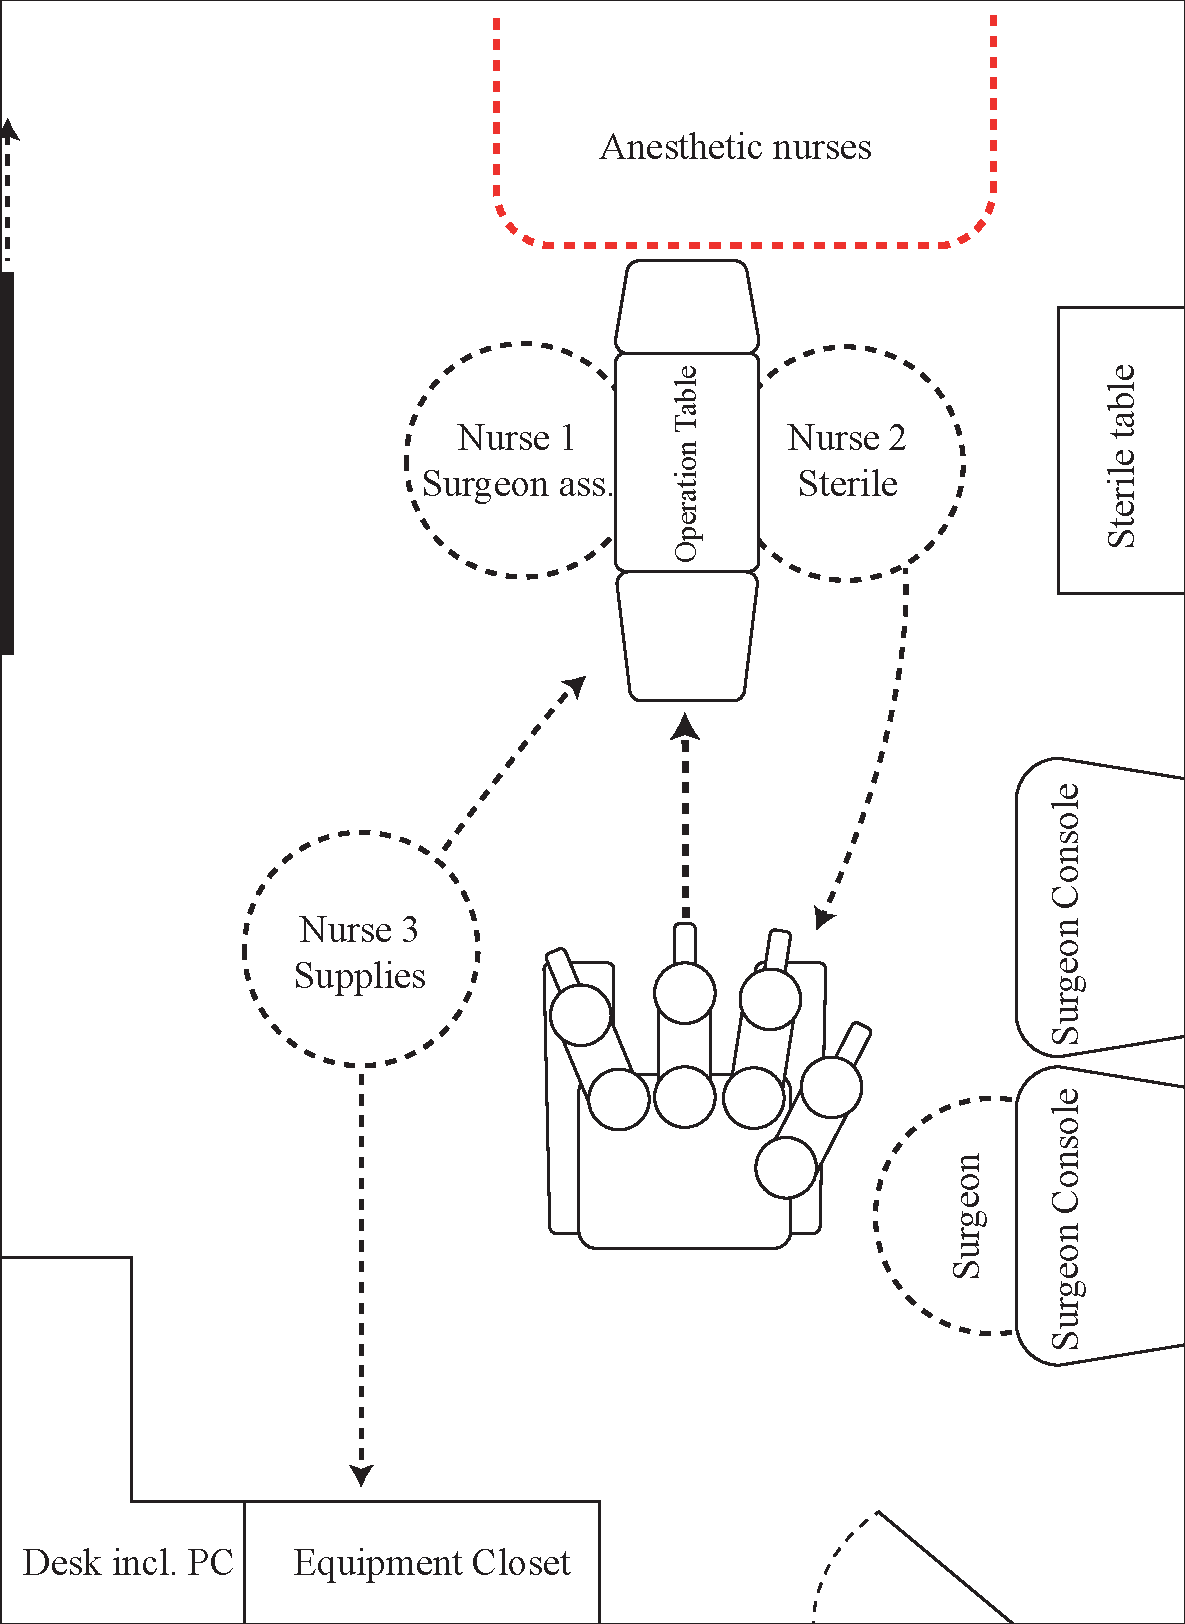
\includegraphics[width=0.5\textwidth]{physical}
	\caption{The phyiscal model showing the layout of the operation room}
	\label{fig:layout}
\end{figure}

The physical enables the development and design of the room when creating the simulation.\\

The sequence model is based on Jane Petersson's worksheet used in team training at MUIC. The sequence model is shown in \autoref{fig:sequence}.

\begin{figure}[hbpt]
	\centering
	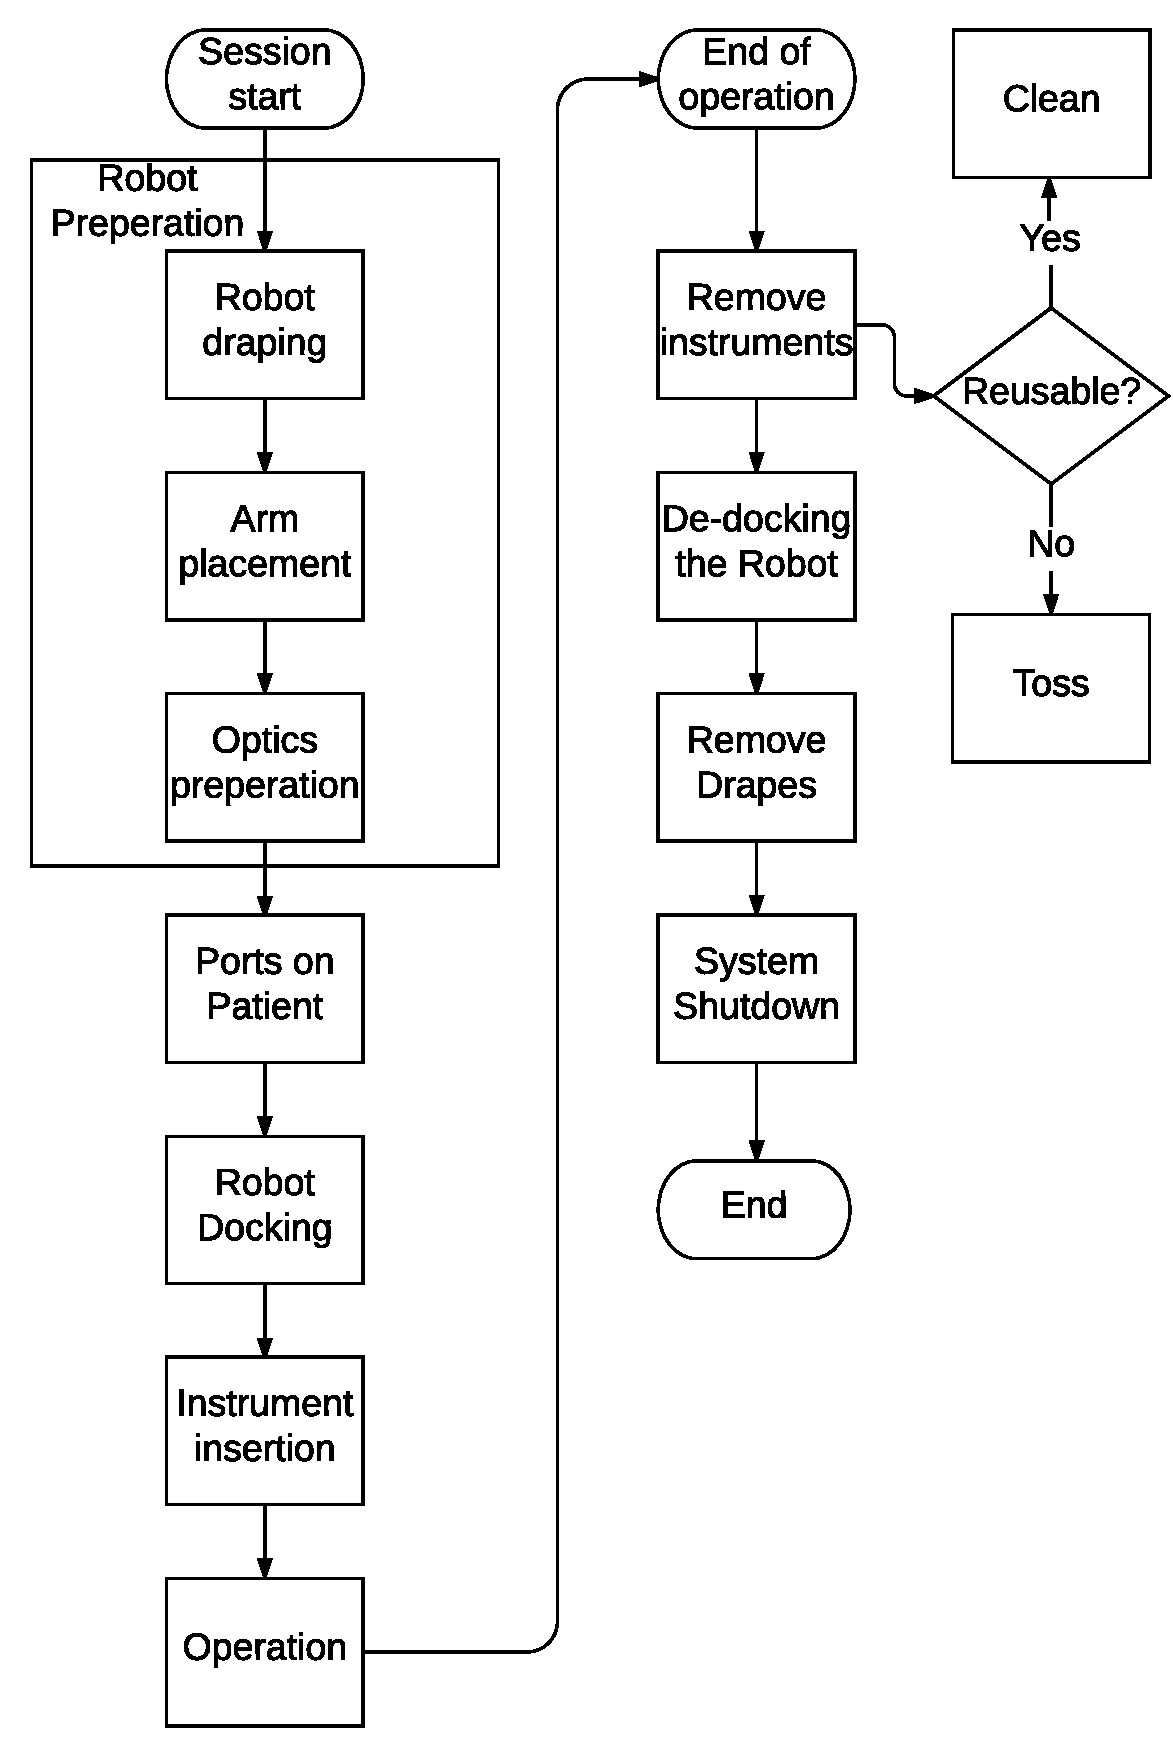
\includegraphics[width=0.4\textwidth]{sequencemodel}
	\caption{Flowchart of the sequence model showing how the operation preparation and debrief is carried out}
	\label{fig:sequence}
\end{figure}

The sequence model describes the actions necessary to both start the operation and to end it. This enables the design of the tasks which should be included in the simulation and their order of appearance to the user.
The model shown is for an operation without any complications, which could lead to de-docking of the robot in an emergency.\\


The Artefact models are shown in figures \ref{fig:drapes}, \ref{fig:camera}, \ref{fig:cam_close}, \ref{fig:port}, and \ref{fig:tools}. These are created from pictures taken during the observation. \autoref{fig:drapes} shows the plastic drapes used to cover the arms of the robot sterilising it. \autoref{fig:camera} shows the endoscopic camera during calibration. \autoref{fig:cam_close} shows the endoscopic camera up close. \autoref{fig:port} shows one of the ports used to insert the tools into the patient. \autoref{fig:tools} shows the tools used with the robot.


\begin{figure}[hbpt]
	\centering
	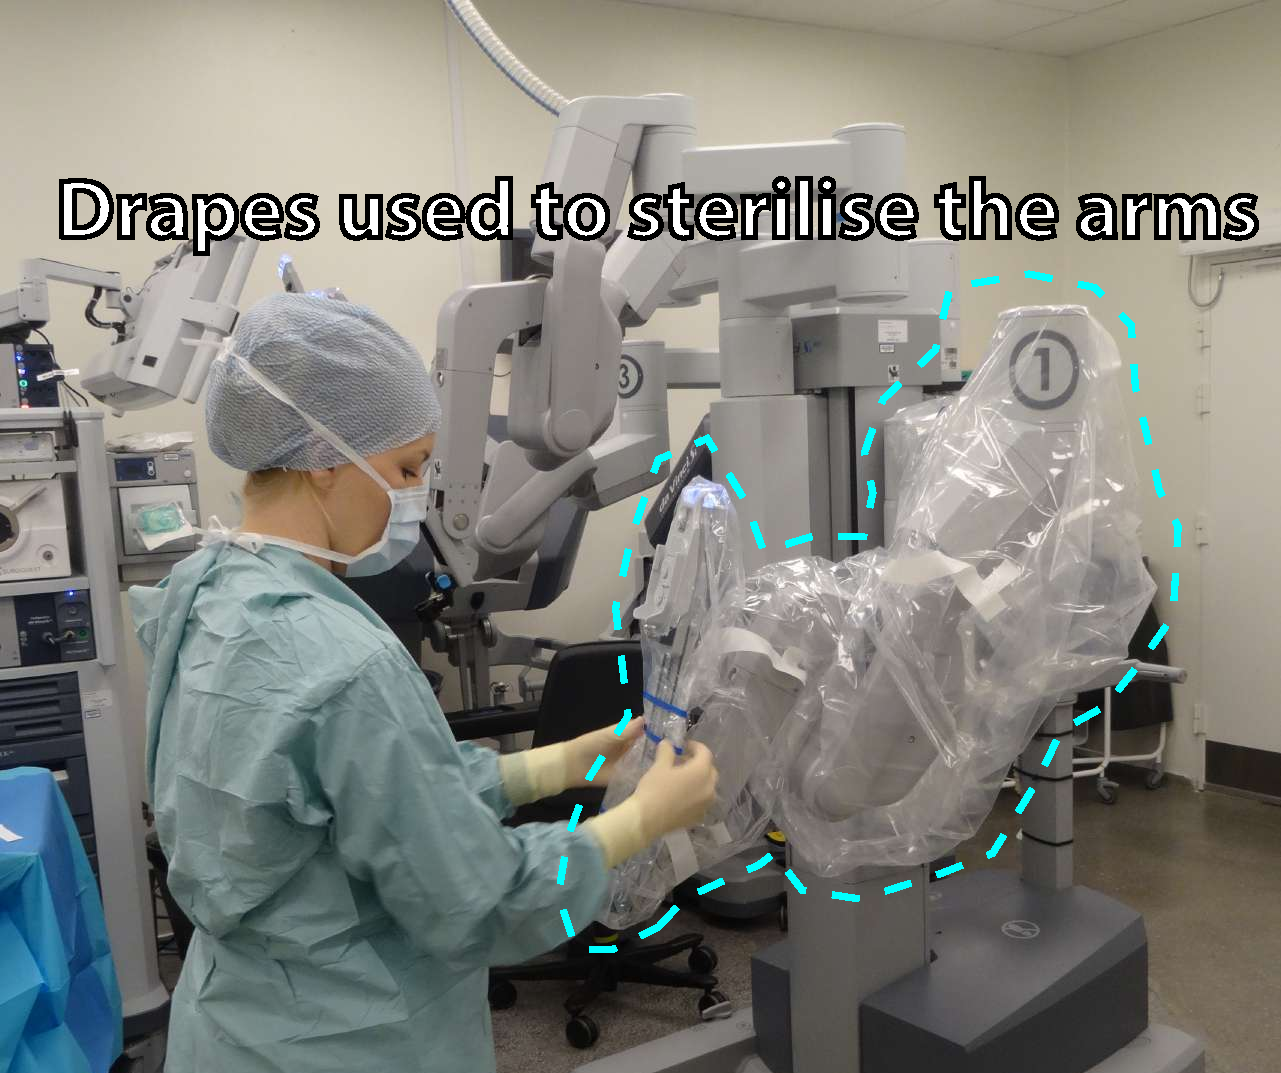
\includegraphics[width=0.4\textwidth]{drapes.pdf}
	\caption{The drapes used to cover the arms of the robot, sterilising them}
	\label{fig:drapes}
\end{figure}

\begin{figure}[hbpt]
	\centering
	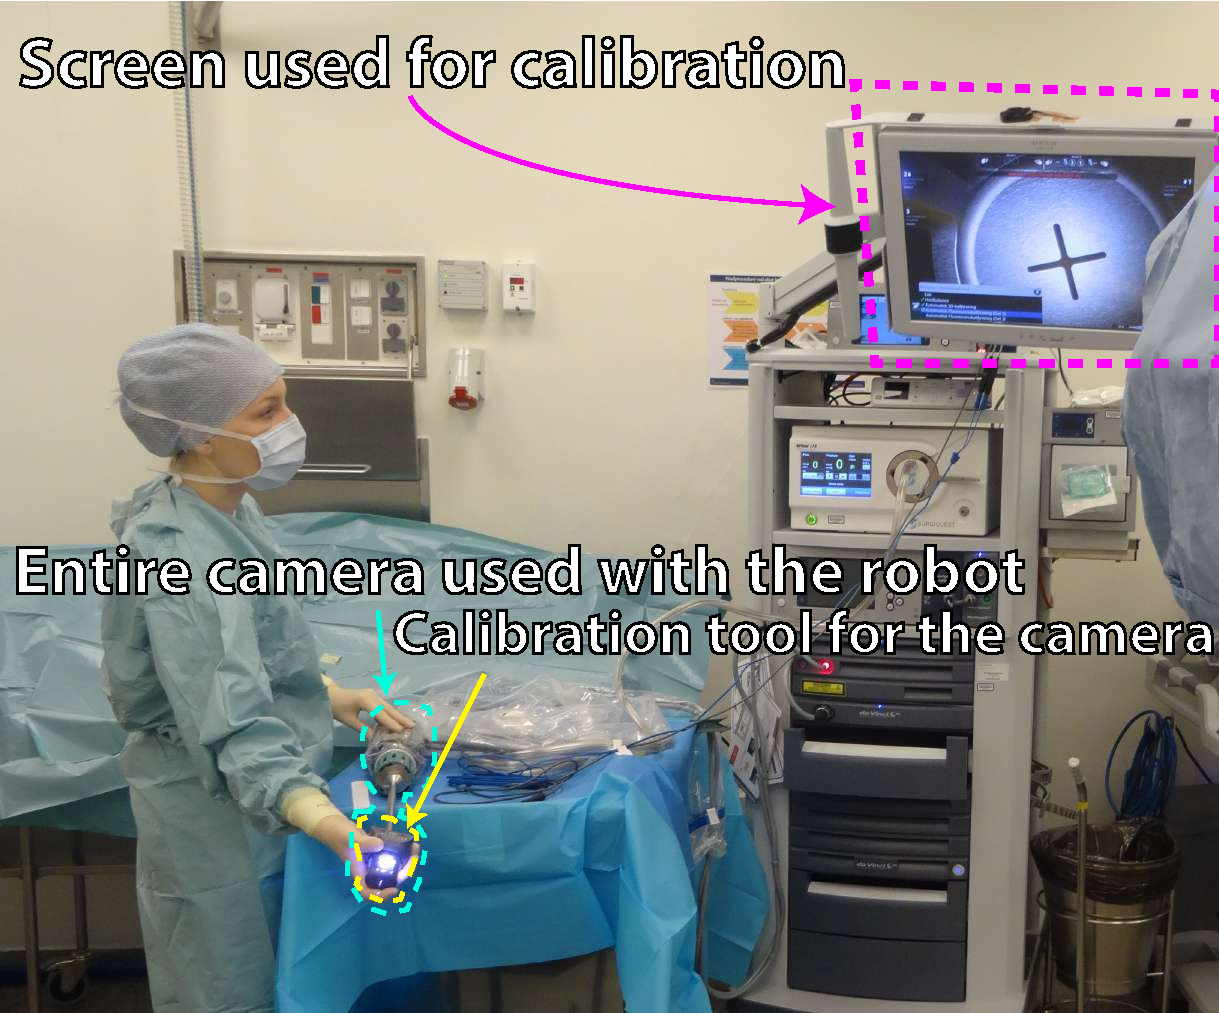
\includegraphics[width=0.4\textwidth]{camera.pdf}
	\caption{The camera used with the robot and a calibration tool}
	\label{fig:camera}
\end{figure}

\begin{figure}[hbpt]
	\centering
	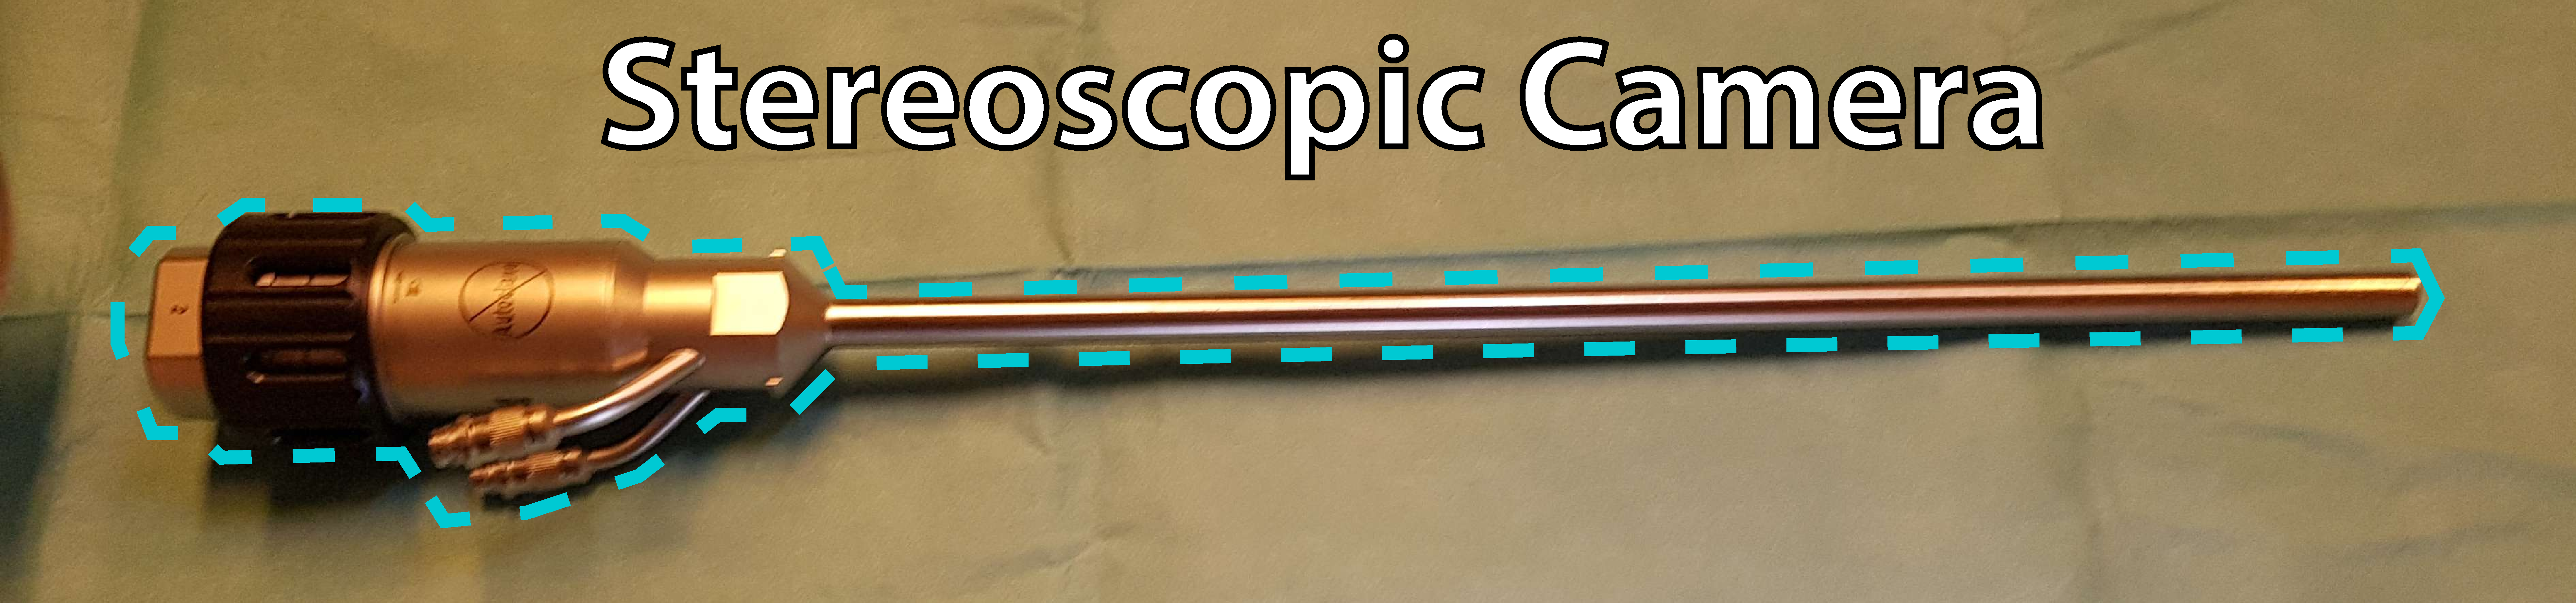
\includegraphics[width=0.4\textwidth]{camera_close}
	\caption{The endoscopic camera up close}
	\label{fig:cam_close}
\end{figure}

\begin{figure}[hbpt]
	\centering
	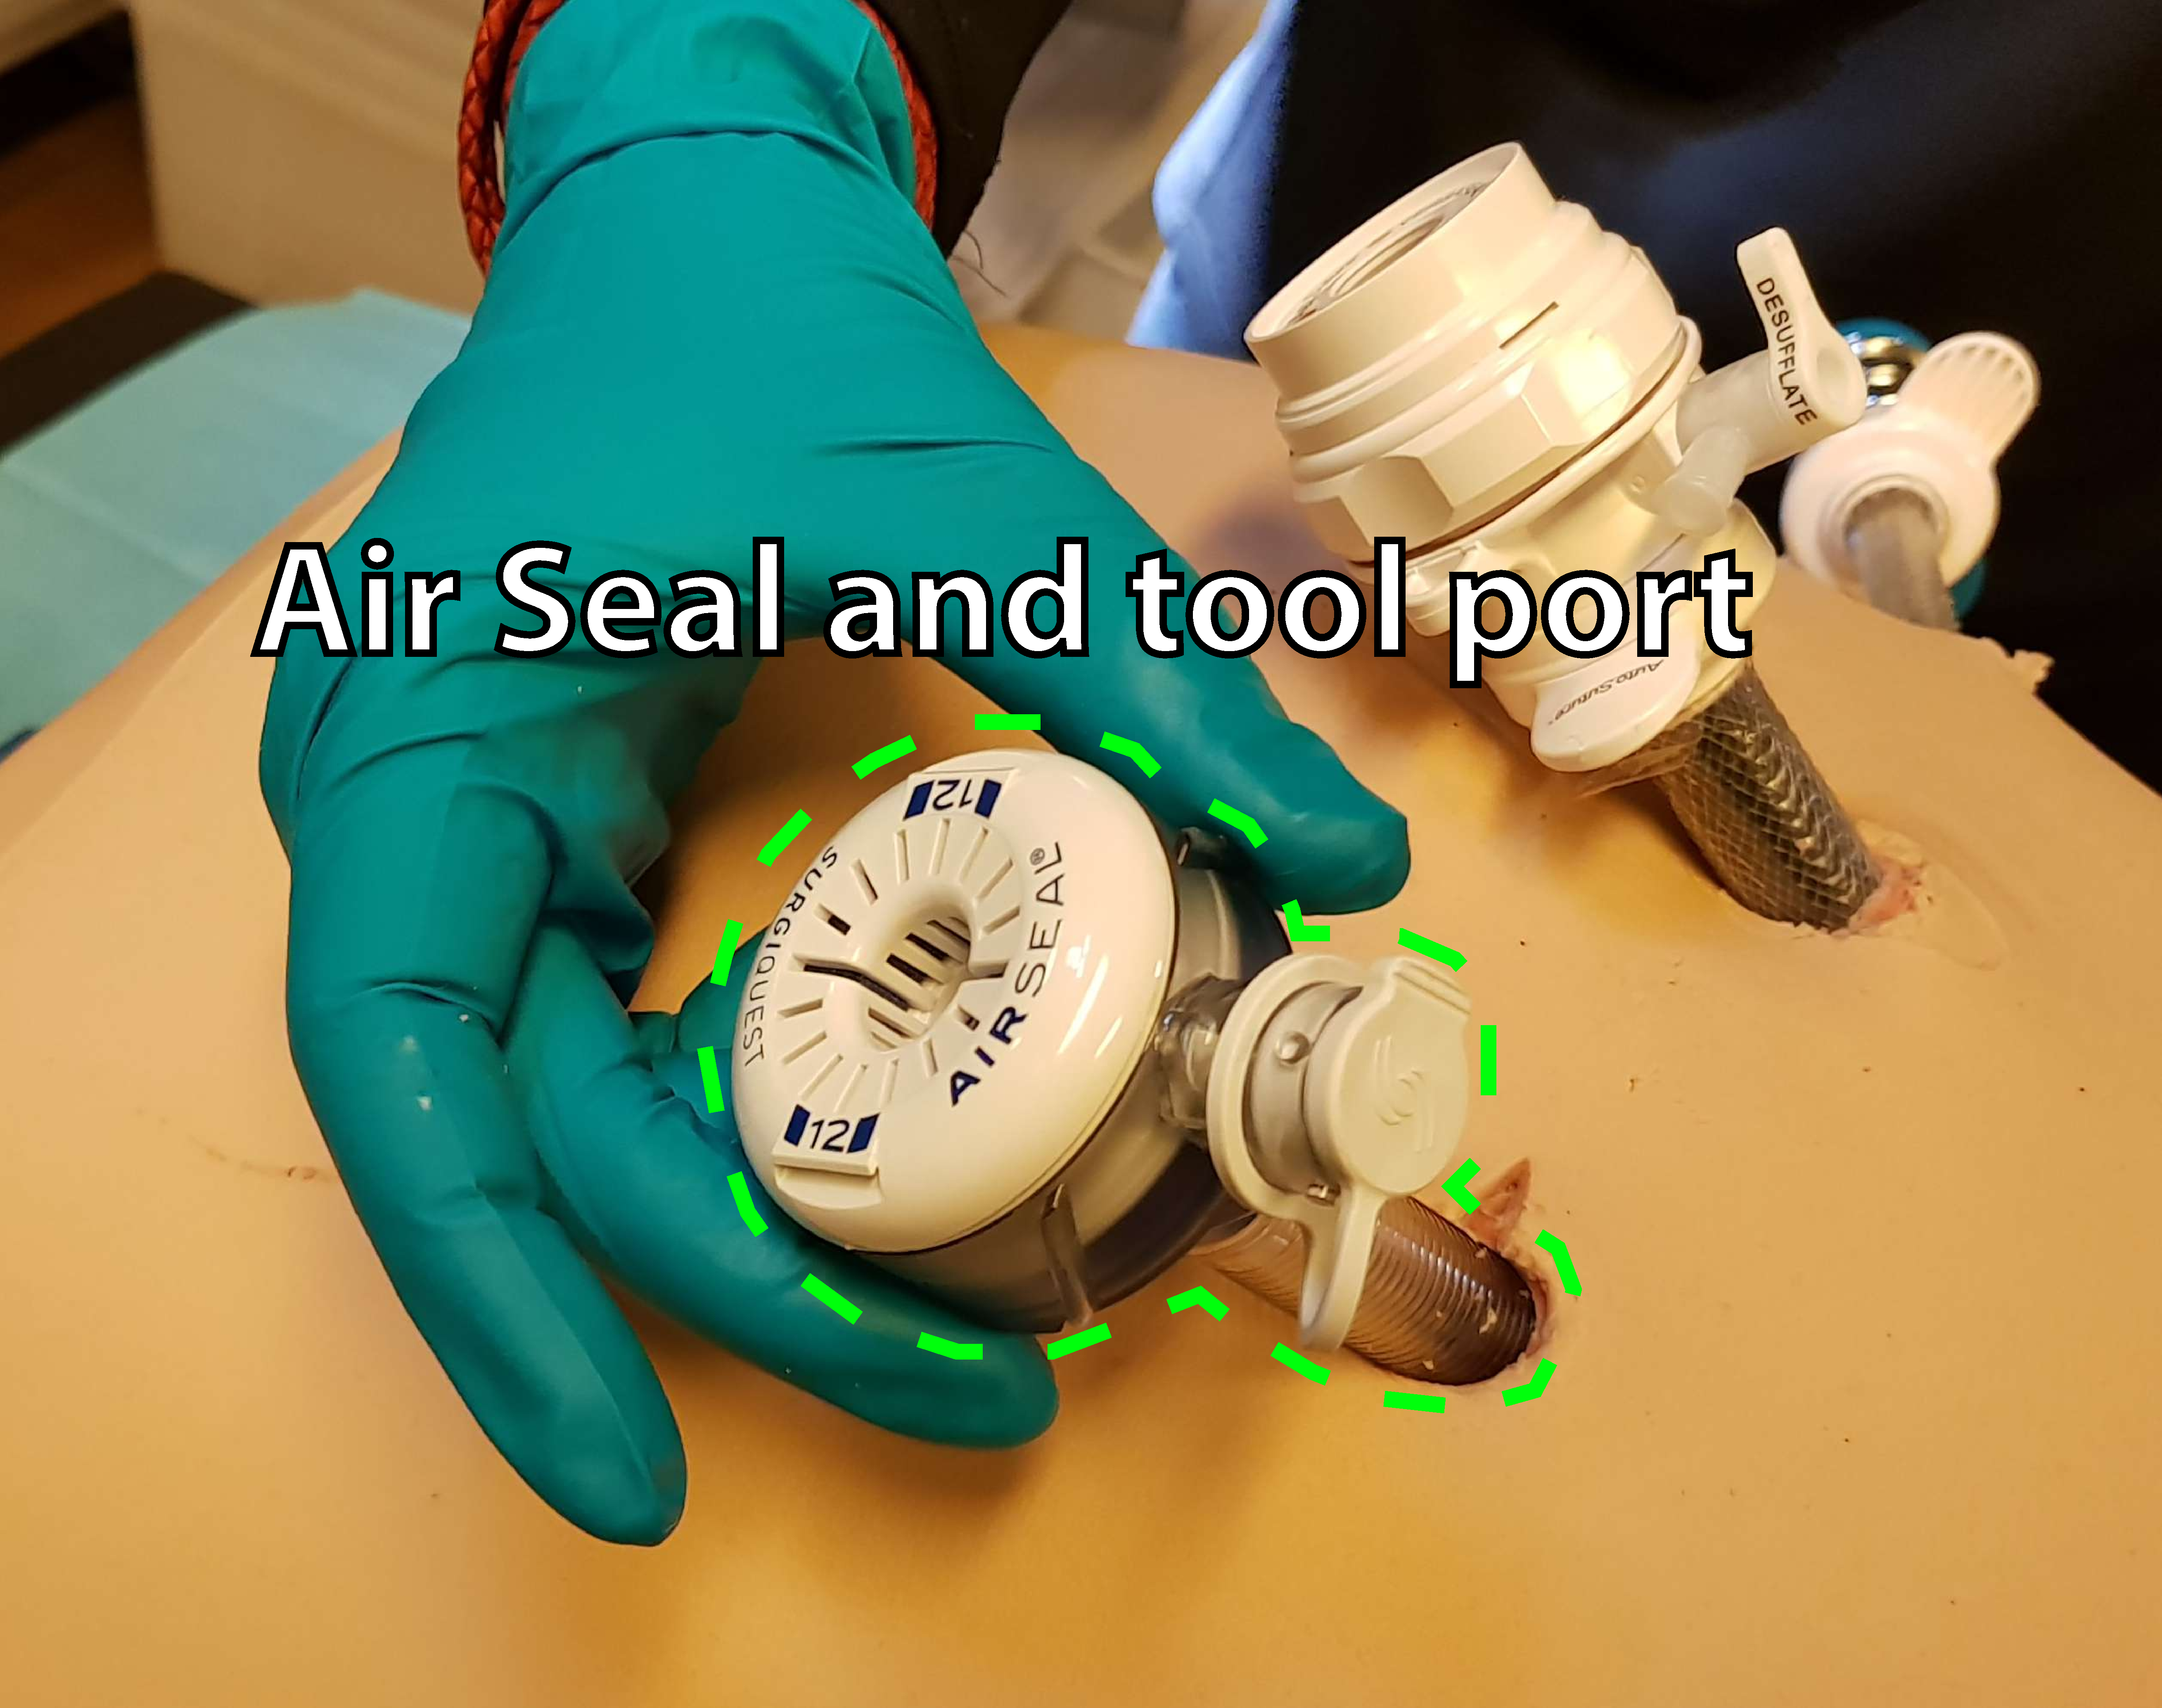
\includegraphics[width=0.4\textwidth]{port}
	\caption{One of the ports used to insert the tools in the patient}
	\label{fig:port}
\end{figure}

\begin{figure}[hbpt]
	\centering
	
\includegraphics[width=0.4\textwidth]{tools}
	\caption{The tools used with the robot}
	\label{fig:tools}
\end{figure}


\subsection{Expert Review}
Jane Petersson and Johan Poulsen were both able to test the system. The following interview revealed that the system at present was satisfactory at simulating the scenario, but was not comprehensive enough to warrant implementation with them. They believed the interaction was sufficient, and that trainees didn’t require additional features, however they both stated that several features should be available to the instructors, such as scene change and reset, interacting with procedures and progress, as well as changing the rules during play (for example by introducing emergencies).

One key point throughout the interview was realism. This was brought up many times during the interview, and the consensus was that the closer the simulation was to total realism, both with controls, models, and textures, the more it could replace or improve upon current training standards. This meant that, for example, the robot should have multiple end effectors to allow more realistic movement. The current da Vinci model has three control points and can rotate around itself which the simulated model does not. In addition, the robot itself should be moveable. Introducing tool ports would, together with the improved handling, allow for teaching docking and undocking in VR. Despite all this, draping the robot arms would need to be practiced at real facilities due to the need for accurate tactile feedback.

Johan Poulsen stated that there were limitations, but that systems such as this could be a must-have for the future of RAMIS. He talked about fully integrating the system with current simulators such as RAMIS console and anaesthetic nurse simulators. This could allow full surgery team training. As noted from the context study, Jane Petersson sabotages the robot setup during team training in order to train the nurses’ and doctors’ communication and emergency handling skills. Being able to control even more factors in virtual reality, such as patient fever, would allow for more detailed training of both nurses and surgeons. This concept could also be extended to include scenarios and scenario control. By being able to reset the scene and load a scenario where the setup is an appendectomy would also improve the utility of the system thereby having multiple scenarios to choose from.

Despite its limitations, the current version could be used to introduce medical students to RAMIS if realism was improved. Johan Poulsen also mentioned that, as there was no tactile feedback, the visuals in the scene had to become more realistic as the vision would overcompensate for the lack of tactile feedback. 

Despite the current limitations both experts agreed that the controls of the system were intuitive and that the learning curve was appropriate for their level of expertise with VR. Observations also showed that they both learned to teleport, grab, and interact with the robot fast.


\section{Conclusion}
The observations and interviews have given an insight as to how both the surgeons and the nurses train and work with the da Vinci Surgical System. Furthermore, critical procedures have been explained by Jane Petersson. These procedures are a must know as failures within these could prove critical or even fatal.\\

The concept of introducing VR training in established RAMIS training sessions seems feasible, however with some caveats. Currently, the system is too basic to warrant implementation at MIUC according to Johan Poulsen, but could serve other purposes such as introducing medical students to RAMIS. Experts stated that the system would require a high level of realism to accurately show the procedure and be useful in RAMIS training.


\end{document}